\chapter{Background \label{ch:background}}
This chapter aims to give an introduction into the \acf{BEXUS} programme as a whole and the \acf{SETH} experiment as a part of this programme. Next the need for the \acf{ADS} is motivated and the measurement methods of the accelerometer and magnetometer explained.

\section{\acs{SETH} and the \acs{BEXUS} programme \label{sec:bg:seth_and_bx_programme}}

The first balloon of the \ac{BEXUS} programme, \textit{BEXUS 1}, launched on November 25$^{\mathrm{th}}$ 2002 at 15:53 UTC. Since then every year, except for 2003, 2020 and 2022, saw balloons being launched from the designated launch site \ac{ESRANGE} near the Swedish city of Kiruna \cite{IAC-08.E.1.1.4}\cite{bexus-campaign-history}.
The \acf{BX} programme is a bilateral programme between the \acf{DLR} and \acf{SNSA}. It offers university student teams the opportunity to build their own experiment and have it fly on a stratospheric balloon. The programme spans around one year and is constructed as a scaled-down version of a real space mission. The \acf{SETH} takes part in the 16th \ac{BEXUS} cycle and is expected to fly between the 3$^\mathrm{rd}$ of October 2025 and 13$^\mathrm{th}$ of October 2025 form \ac{ESRANGE}.

The purpose of \ac{SETH} is to investigate the angular dependency of particle radiation in the upper atmosphere. To this end a means of measuring the experiments attitude and heading while on the gondola is required.

The main source of radiation in the atmosphere are \acp{GCR} that hit the earth isotropically from all directions. In 1935 Erich Regener and Georg Pfotzer published an article in \textit{Nature} presenting a figure (see fig. \ref{fig:regener1935}) which shows the radiation intensity measured by three Geiger-Müller Counters stacked on top of each other two have an aperture angle of about 20$^\circ$ around the zenith \cite{regener-pfotzer-1935}.

\begin{figure}[H]
    \centering
    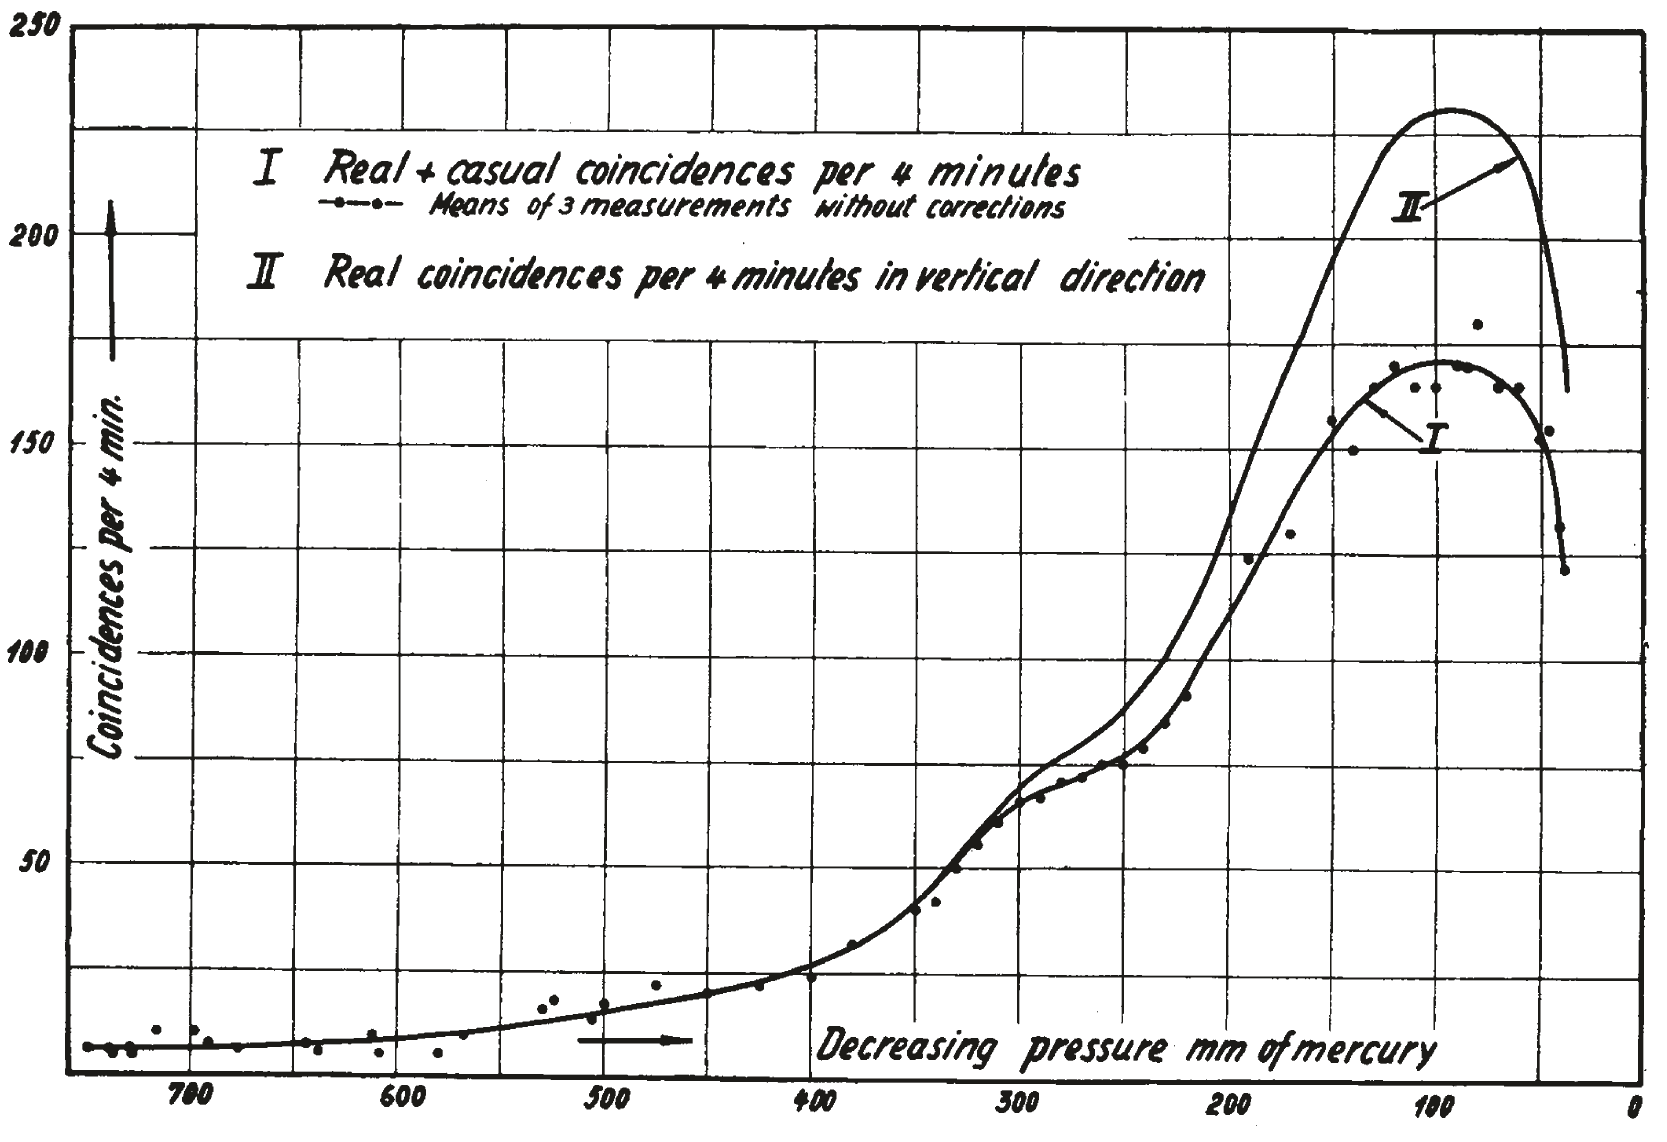
\includegraphics[width=0.8\linewidth]{images/01_background/original_regener_pfotzer.png}
    \caption[Regener-Pfotzer-Maximum as shown in \cite{regener-pfotzer-1935}]{Curve I shows the uncorrected coincidences per 4\,min. against ambient pressure in mm\ce{Hg}. Curve II shows the corrected coincidences taking the probability of coincidence counting against casual coincidences into account.}
    \label{fig:regener1935}
\end{figure}

Eighty Years later, the \ac{ADAM} \ac{BEXUS} Team around Dennis Trautwein showed that the fluence of particles for a given altitude varied with the zenith angle. Figure \ref{fig:martensen2015} taken from \cite{martensen2015} shows the angular distribution of particle fluence at an altitude of 27\,km.

\begin{figure}[H]
    \centering
    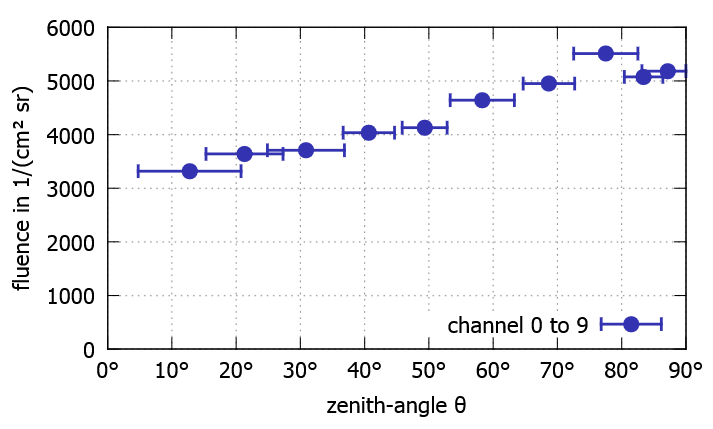
\includegraphics[width=0.6\linewidth]{images/01_background/martensen.png}
    \caption[Results of \acs{ADAM} at 27\,km]{Angular distribution of the charged particle fluence at an altitude of 27\,km.}
    \label{fig:martensen2015}
\end{figure}

Counting rate $C$ (coincidences per unit time) and isotropic Intensity $I_0$ (Fluence per unit time) share a linear relationship with the Geometrical Factor $G$ as coefficient, as is given in eq. \eqref{eq:sullivan}\cite{SULLIVAN19715}.
\begin{equation}
    C=G\cdot I_0
    \label{eq:sullivan}
\end{equation}

The goal of \ac{SETH} is to measure the angular distribution of the Regener-Pfotzer-Maximum in the zenith angle and additionally in the azimuthal angle. A \ac{CAD} model of parts of the \ac{SETH} detector is shown in fig. \ref{fig:seth_cad}. The zenith and azimuthal angle of an incoming particle can be determined through the coincidence of two photodiodes (active area shown in orange).

\begin{figure}[H]
    \centering
    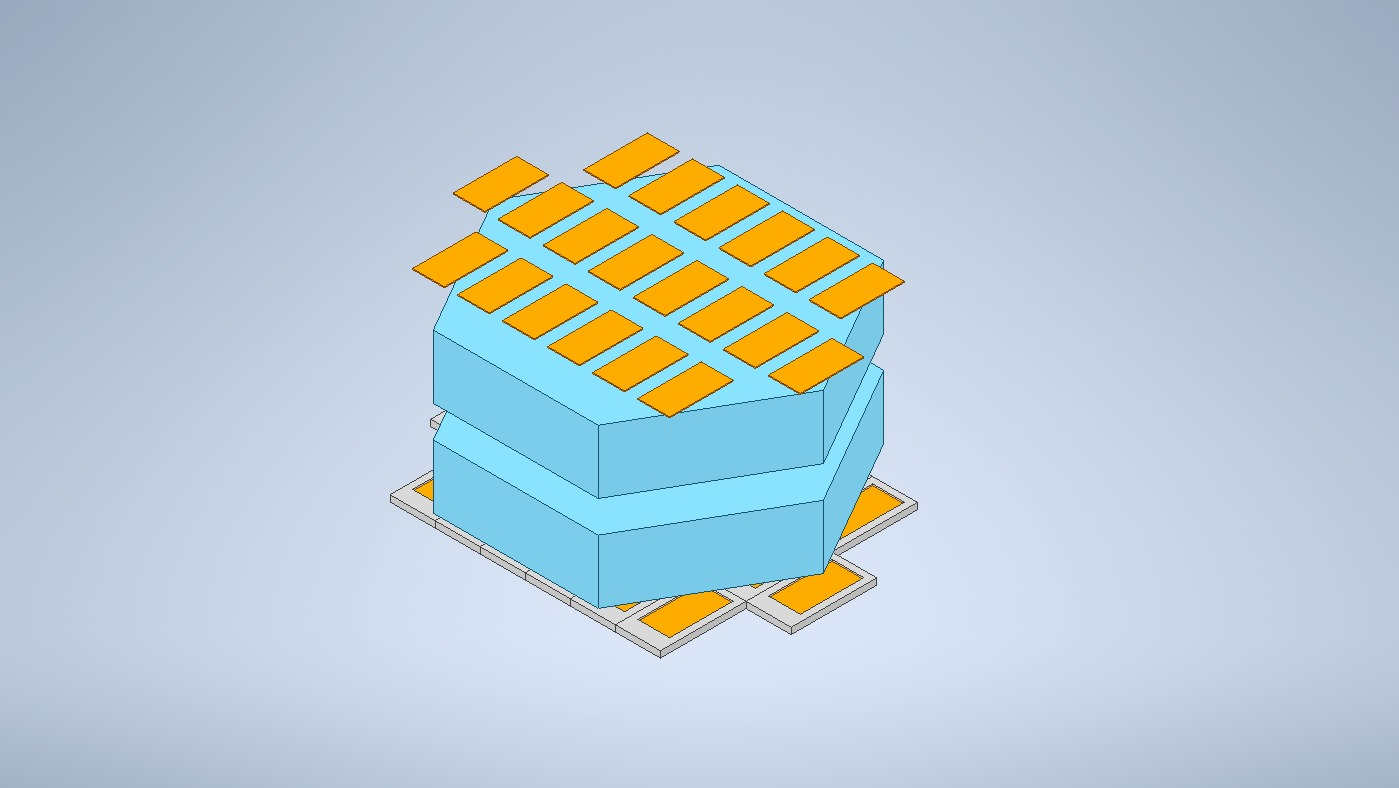
\includegraphics[width=0.5\linewidth, trim = {5cm 0cm 5cm 0cm}, clip]{images/01_background/SETH-Sketch.jpeg}
    \caption[\ac{SETH} detector sketch]{\ac{CAD} model of the \ac{SETH} detector showing the array of diodes.}
    \label{fig:seth_cad}
\end{figure}

The gondola hanging from the \ac{BEXUS} balloon does not have a fixed orientation in space. The wind will incite the gondola to rotate and swing during all phases of flight. Thus to get a reliable measurement of the angular distribution of the Regener-Pfotzer-Maximum in the azimuth domain, accurate heading information is required so as to know which direction particles travelling through the telescope hail from. The heading may occasionally be called yaw or azimuth.

\framebox[\linewidth][c]{\textbf{Objective 1.: The gondolas heading shall be measured.}}

As mentioned above, the gondola will also experience swinging or more accurately pitching and rolling. This is a deflection from the plane parallel to the local earths surface, split into the lateral and longitudinal axis of the gondola (see fig. \ref{fig:attitude}). As the gondola is a rigid body and all experiments are fixated, the attitude of the gondola as a whole is the same as the attitude of our experiment.

\framebox[\linewidth][c]{\textbf{Objective 2.: The gondolas attitude shall be measured.}}

\begin{figure}[H]
    \centering
    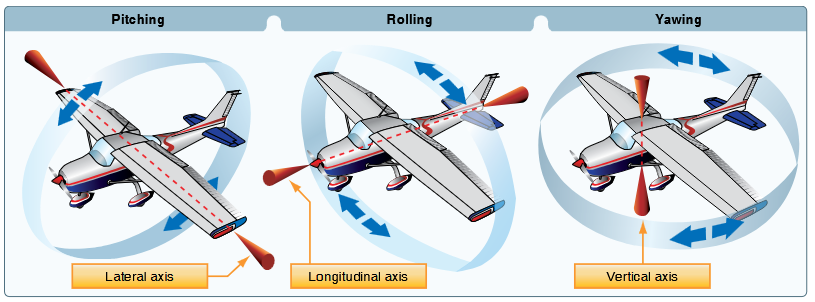
\includegraphics[width=0.5\linewidth]{images/01_background/axes_of_an_airplane.png}
    \caption[Axes of an airplane]{Axes of an airplane, taken from \cite{pilot-handbook}.}
    \label{fig:attitude}
\end{figure}

It is the job of the \ac{ADS} to fulfil objectives 1 and 2. Thus this thesis will cover the implementation, calibration and preliminary testing of the \ac{ADS}.

\section{Accelerometers \label{sec:bg:accelerometers}}
The typical accelerometer is a \ac{MEMS}

\section{Magnetometers \label{sec:bg:magnetometers}}
To determine the gondola's heading, a magnetometer is used just like a compass. While many phenomena can be used to determine the magnitude and direction of a magnetic field, the sensor used for this thesis relies on tunnel magnetoresistance.